% Scientific Reports submission (Springer Nature template, sn-nature reference style)
% Revised manuscript: method on measured outputs, biological/calibration split, re-estimation
% criterion, backward elimination, external validation, robustness, cost and formal guarantees.
% Figures: make_figures.py; Table 1 and Supplementary Table S1: make_tables.py.

\documentclass[pdflatex,sn-nature]{sn-jnl}

\usepackage{graphicx}
\usepackage{multirow}
\usepackage{amsmath,amssymb,amsfonts}
\usepackage{amsthm}
\usepackage{booktabs}
\usepackage{xcolor}
\usepackage{url}
\usepackage{lineno}
\linenumbers
\raggedbottom

\theoremstyle{plain}
\newtheorem{theorem}{Theorem}

\begin{document}

\title[Few biological parameters reproduce measured dynamics]{Few biological parameters suffice to reproduce measured dynamics in systems biology models: local sensitivity-based reduction with formally verified mathematical guarantees}

\author*[1]{\fnm{M\'onica} \sur{Miranda R.}}\email{mmmirand@espol.edu.ec}
\author[1]{\fnm{Carlos} \sur{Salazar}}\email{asalazar@espol.edu.ec}
\author[1]{\fnm{C\'esar} \sur{Mart\'in}}\email{cmartin@espol.edu.ec}
\author[1]{\fnm{Adriana} \sur{Aguirre}}\email{aaaguirr@espol.edu.ec}

\affil*[1]{\orgdiv{Faculty of Engineering, Control and Automation Systems Group}, \orgname{Escuela Superior Polit\'ecnica del Litoral (ESPOL)}, \orgaddress{\city{Guayaquil}, \country{Ecuador}}}

\abstract{Mathematical models of biological processes often contain dozens to hundreds of unknown rate constants, but experimental data rarely contain enough information to estimate all of them. We present a method that, before any model fitting, identifies a small set of biological parameters that is sufficient to reproduce the measured data when only those parameters, together with the measurement scaling and offset factors, are re-estimated and all other parameters are kept at their published values. The method ranks parameters by how strongly they change the measured quantities, discards parameters whose effects are redundant, checks that the reduced model can reproduce the data under random parameter perturbations, and finally removes any parameter that is not needed. We applied it to 34 published models with real experimental data. In 32 of them, a small subset was sufficient, in most cases only two biological parameters. When fitted to part of the experiments, the reduced models predicted the remaining experiments as well as or better than the full models in 24 of 25 testable cases, and most remained adequate for parameter changes of up to 50\%. The cost grows linearly with model size. Its main mathematical steps are verified with a computer proof assistant.}

\keywords{parameter reduction, practical identifiability, sensitivity analysis, ordinary differential equations, systems biology, formal verification}

\maketitle

% Scientific Reports: single-column, unjustified text
\raggedright
\setlength{\parindent}{1.5em}

\section*{Introduction}\label{sec:intro}

Ordinary differential equation (ODE) models are central to quantitative biology, pharmacology and epidemiology, where they describe how interacting molecular species or populations change over time as a function of kinetic parameters $\theta$\cite{bib16}. Using a model for prediction requires estimating $\theta$ from experimental measurements, and this becomes difficult as models grow. The main obstacle is non-identifiability: different parameter values may produce the same measured output, either because of model symmetries (structural non-identifiability) or because the available data are insufficient (practical non-identifiability)\cite{bib4,bib10,bib29}. In both cases the likelihood has flat ridges on which optimisers stall and confidence intervals become unreliable\cite{bib24,bib25,bib17}. Models in public benchmark collections routinely contain 20--300 parameters\cite{bib31}, and genome-scale models contain thousands\cite{bib12}.

The sloppy-model phenomenon offers a structural explanation\cite{bib15}: the sensitivity of model outputs to parameters is typically dominated by a few ``stiff'' directions, while many ``sloppy'' directions have almost no effect on the outputs. This suggests that a small subset of parameters may suffice to describe what is actually measured. Exploiting this observation in practice requires answering three questions that existing tools address only partially. First, which parameters should be retained? Sensitivity indices\cite{bib26,bib23} and profile likelihoods\cite{bib24} rank parameters by importance, but they do not ensure that the retained parameters are mutually non-redundant, so the reduced estimation problem may still be ill-conditioned\cite{bib5,bib9}. Second, is the reduced model good enough? A reduction is useful only if re-estimating the retained parameters reproduces the measured data and predicts experiments that were not used for fitting. Third, how much can the conclusions be trusted? Statements such as ``the discarded parameters can be fixed'' rest on approximations whose validity is rarely made explicit.

This work was motivated by a dynamical model of Bandura's social cognitive theory\cite{bib3,bib34}, in which six psychosocial constructs that determine physical activity interact through 22 parameters (coupling strengths, input gains and time constants). When all 22 parameters were estimated from 31 days of step-count data, many stable parameter sets fitted the data with widely different quality (coefficients of determination between 4\% and 86\%), and local refinement from the best global estimate lowered the fit from 86\% to 41\%\cite{bib35}. Such behaviour is typical when several parameters have nearly identical effects on the measured output, so that the data cannot separate them; in such models, a principled way to decide which parameters to estimate is indispensable.

Here we present a reduction method that works directly on the measured outputs defined in the PEtab format\cite{bib27}, including experimental conditions, measurement transformations and noise levels. It distinguishes biological parameters, which belong to the mechanistic model, from calibration parameters (scaling factors and offsets of the measurement process), which are always re-estimated, and selects only among the biological ones. Candidates are ranked by sensitivity, redundant candidates are rejected by condition-number and variance-inflation tests, the reduced model is accepted only if re-estimating its parameters reproduces the full model under random parameter perturbations, and a final backward elimination makes the subset minimal with respect to inclusion. We evaluate the method on 34 benchmark problems with real data\cite{bib31,bib27}, test the reduced models on held-out experiments, quantify their robustness to perturbation size and to the method's own settings, and report the computational cost. The main mathematical statements on which the method relies are formally verified in the Lean~4 proof assistant with the Mathlib library\cite{bib19,bib21}; we state precisely what is and what is not proved.

\section*{Results}\label{sec:results}

\subsection*{Overview of the method}\label{sec:overview}

Figure~\ref{fig:pipeline} summarises the procedure; all symbols are defined in the Methods and in Supplementary Table~S2. The input is a PEtab problem: an SBML model, the list of measured observables with their experimental conditions, measurement times, transformations (linear, logarithmic) and noise standard deviations $\sigma_i$, and the nominal parameter values $\theta_0$ reported by the original authors. Each measurement $i$ defines a scaled output $y_i(\theta)=h(g_i(x(t_i;\theta),\theta))/\sigma_i$, so that all outputs are comparable in units of measurement noise. Parameters are split into biological parameters $\theta_B$ (those of the SBML model) and calibration parameters $\theta_C$ (observation scalings and offsets); only biological parameters are candidates for selection, while calibration parameters are always re-estimated together with the selected ones.

The relative sensitivity matrix $J=\partial y/\partial\log\theta$ is computed once at $\theta_0$ by central finite differences. In stage~1, biological parameters are added in decreasing order of their sensitivity energy $E_j=\|J_{:,j}\|^2$; a candidate is accepted only if the condition number $\kappa$ and the largest variance inflation factor (VIF) of the normalised columns of $J_S$ stay below a threshold, and is otherwise discarded permanently. Stage~1 stops when the accepted parameters capture a fraction $\tau_R$ of the total energy. The resulting subset $S$ is then tested: in random scenarios where all parameters are perturbed, $\theta_S$ and $\theta_C$ are re-estimated with the remaining parameters fixed at $\theta_0$, and $S$ is admissible if the median relative fitting error $e_{\mathrm{fit}}$ is below $\tau_e$ and $|S|\ge 2$. The threshold $\tau_e=\sqrt{1-c^2}$ equals the smallest error attainable by rescaling an output change whose cosine similarity with the full change is $c$ (Theorem~\ref{thm:cos}); we use $c=0.9$, so $\tau_e=0.436$. If stage~1 does not yield an admissible subset, stage~2 repeats the selection with parameters ordered by their finite-perturbation effect $s_j$ until an admissible subset is found. Finally, backward elimination removes any parameter whose removal keeps the subset admissible, which yields a subset that is minimal with respect to inclusion (Theorem~\ref{thm:prune}).

\begin{figure}[t]
\centering
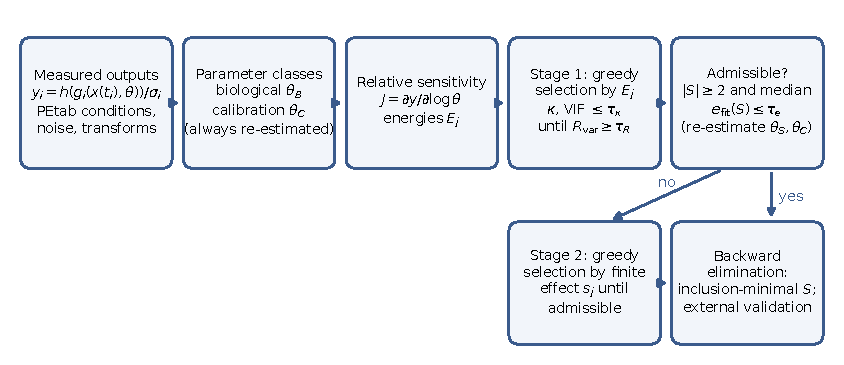
\includegraphics[width=\textwidth]{figures/fig1_pipeline.pdf}
\caption{\textbf{Overview of the reduction method.} Measured outputs are scaled by their noise level; biological and calibration parameters are separated; the relative sensitivity matrix $J$ is computed at the nominal parameters. Stage~1 selects biological parameters in decreasing order of sensitivity energy, rejecting candidates that make the selection ill-conditioned ($\kappa$ or VIF above $\tau_\kappa$), until a fraction $\tau_R$ of the energy is captured. The subset is admissible if re-estimating it, together with the calibration parameters, reproduces the full model in random perturbation scenarios (median $e_{\mathrm{fit}}\le\tau_e$) and it has at least two parameters. Otherwise stage~2 repeats the selection ordered by finite-perturbation effects. Backward elimination then removes unnecessary parameters, and the reduced model is validated on held-out experiments.}
\label{fig:pipeline}
\end{figure}

\subsection*{A motivating case with exact collinearity}\label{sec:sct}

The social cognitive theory model\cite{bib3,bib34,bib35} describes how six psychosocial constructs, such as self-efficacy, perceived barriers and behaviour, respond to six external inputs through a linear system $\tau_i\dot x_i=-x_i+\sum_j\beta_{ij}x_j+\sum_k\gamma_{ik}u_k$ with 22 parameters (six time constants $\tau_i$, ten couplings $\beta_{ij}$ and six input gains $\gamma_{ik}$); the measured output is behaviour (daily steps). We analysed it at the parameter values previously estimated for one participant\cite{bib35}, with each input excited in turn (Methods). It is not counted in the benchmark below because no experimental data set is used here. With behaviour as the only output, the 22 parameters cannot all be estimated even from noise-free data: the sensitivity matrix is exactly rank-deficient (infinite condition number), and 51 pairs of parameters have sensitivity vectors with cosine similarity of at least 0.95, several equal to 1.000 (for example $\beta_{14}$, $\beta_{21}$ and $\beta_{31}$, or $\beta_{25}$ and $\beta_{42}$). This is expected for a single output of a linear system, whose response is determined by fewer combinations of parameters than there are parameters. The method selected two parameters, $\beta_{45}$ and $\beta_{43}$; the conditioning test rejected 14 candidates, for example $\beta_{54}$, $\tau_1$ and $\tau_2$ (cosine 0.99 with $\beta_{45}$) and $\tau_3$ (0.99 with $\beta_{43}$). Re-estimating only these two parameters reproduced the output with a median $e_{\mathrm{fit}}$ of 10.8\% at $\pm$5\%, and the error stayed between 9.4\% and 11.0\% for perturbations up to $\pm$50\% (pattern A). When all six constructs are treated as outputs, the full parameter set becomes identifiable in principle but remains ill-conditioned (condition number 202, nine pairs with cosine $\ge 0.95$), and the method selects $\beta_{45}$ and $\beta_{14}$ ($e_{\mathrm{fit}}=27.2\%$, pattern A).

\subsection*{Benchmark: a few biological parameters suffice in most models}\label{sec:benchmark}

We applied the method to 34 PEtab benchmark problems with real measurements\cite{bib31,bib27} covering signalling, metabolism, gene regulation, cell cycle, immunology and epidemiology, with 3 to 294 parameters and 16 to 27,132 measurements (Table~\ref{tab:benchmark}). One further benchmark problem (Froehlich, 4,231 parameters and 9,169 experimental conditions) was analysed only on its state trajectories because each evaluation of its measured outputs requires about 9,000 simulations; it is not counted here (see Computational cost).

The method found an admissible subset in 32 of the 34 problems (Fig.~\ref{fig:benchmark} and Table~\ref{tab:benchmark}). In 29 of them the subset contains only two biological parameters; the remaining three contain three (Zhao), five (Bruno) and ten (Lucarelli). Sixteen problems also have calibration parameters (up to 79 in Raimundez), which are re-estimated in every case. Counting both kinds, the reduced estimation problem has a median of 78\% fewer free parameters than the full one (range 33--97\%); among biological parameters alone, the median reduction is 88\%. Backward elimination removed between one and five parameters in seven problems (Supplementary Table~S1). Stage~1 alone was sufficient in seven problems; in the other 25, the energy ordering selected parameters whose re-estimation could not reproduce the full model, and the finite-effect ordering of stage~2 was needed. The two non-admissible problems fail for different reasons. In Crauste, a model of the T-cell response with quadratic proliferation and pathogen-growth terms, the published parameters lie at the edge of a regime in which the solution grows without bound in finite time: changing a single parameter by 1\% (for example, decreasing the effector proliferation rate $\rho_E$ by 1\%) makes the effector populations increase from about $5\times 10^2$ to $5\times 10^5$ cells within four days, after which no solution exists on the measured horizon. This happened for 8--9 of the 24 one-at-a-time perturbations of $\pm$1\% and for 7 of the 15 scenarios at $\pm$5\%, independently of the integrator tolerances (relative tolerances from $10^{-10}$ to $10^{-5}$), so the sensitivity matrix and the admissibility test are not defined and no local reduction method is applicable; consistently, global existence of solutions for this model could only be proved formally on a short horizon ($T\le 1$). In Beer, the selection stopped at 18 parameters because any further parameter violated the conditioning test, and the resulting subset had $e_{\mathrm{fit}}=50\%$, above the threshold.

Re-estimation is essential. When the selected parameters are simply set to their perturbed values, without re-estimation, the median relative error $e_{\mathrm{rel}}$ exceeds $\tau_e$ in 23 of the 32 admissible problems (Fig.~\ref{fig:benchmark}b); after re-estimation the median error $e_{\mathrm{fit}}$ is 14\% (maximum 43.5\%). In other words, the selected parameters do not replicate the effect of every individual perturbation; rather, adjusting them compensates for the perturbations of all other parameters in the measured outputs. This is precisely the property needed when the reduced model is fitted to data.

\begin{figure}[t]
\centering
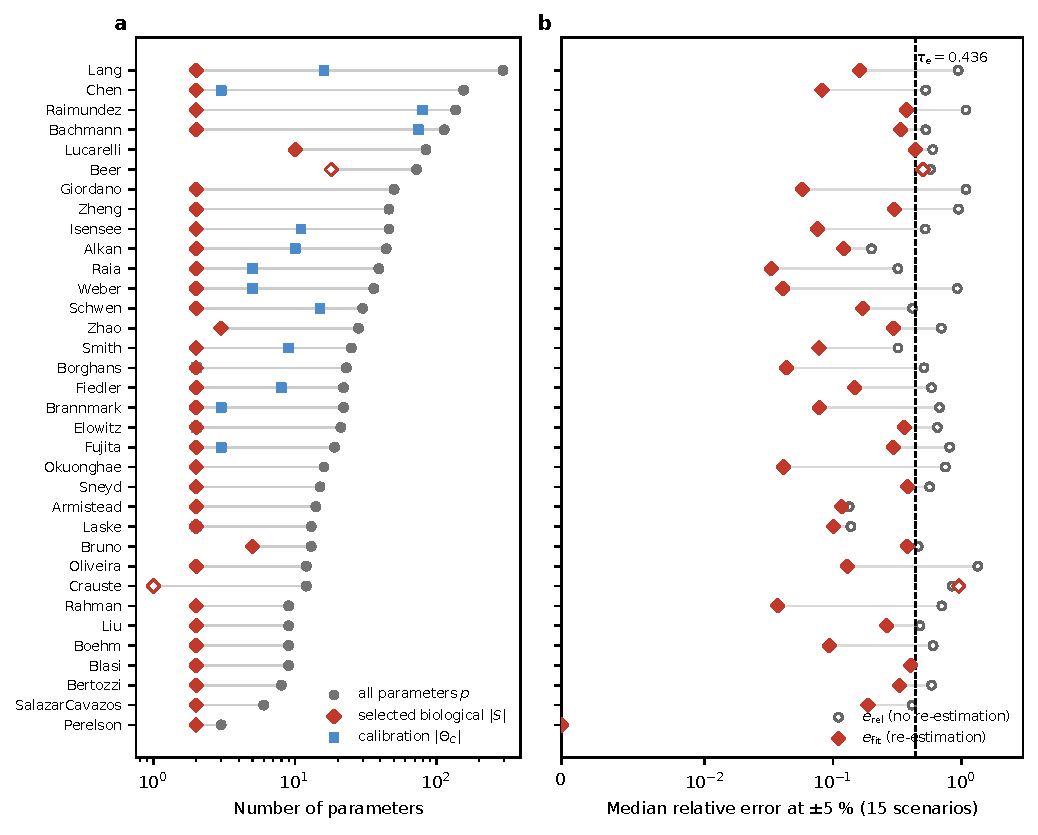
\includegraphics[width=\textwidth]{figures/fig2_benchmark.pdf}
\caption{\textbf{Reduction across 34 benchmark problems.} \textbf{a}, Number of parameters of the full model ($p$, grey circles), calibration parameters that are always re-estimated ($|\Theta_C|$, blue squares) and selected biological parameters ($|S|$, red diamonds; open diamonds, no admissible subset). Problems are sorted by $p$. \textbf{b}, Median relative error over 15 random scenarios at $\pm$5\% when the selected parameters are set to their perturbed values without re-estimation ($e_{\mathrm{rel}}$, open circles) and after re-estimating them together with the calibration parameters ($e_{\mathrm{fit}}$, red diamonds). The dashed line marks the admissibility threshold $\tau_e=0.436$, equivalent to a cosine similarity of 0.9. The horizontal axis is linear below 0.01 and logarithmic above.}
\label{fig:benchmark}
\end{figure}

\begin{table}[t]
\caption{\textbf{Per-problem results.} $p$, number of estimated parameters; $m$, number of measurements; $|\Theta_C|$, calibration parameters (always re-estimated); $|S|$, selected biological parameters; Stage, stage that produced the subset; $e_{\mathrm{rel}}$ and $e_{\mathrm{fit}}$, median relative error over 15 scenarios at $\pm$5\% without and with re-estimation (admissibility: $e_{\mathrm{fit}}\le 43.6\%$; italic, not admissible; $^{\ast}$, $e_{\mathrm{fit}}$ computed to first order because of simulation cost; $^{\dagger}$, not defined because the model has no solution on the measured horizon for 1\% parameter changes); Pattern, robustness pattern over perturbation sizes from $\pm$1\% to $\pm$50\% (see text); Test $\chi^2/n$, mean squared noise-scaled residual on held-out experiments for the reduced and the full model, both re-estimated on the training experiments (values near 1 mean errors of the size of the measurement noise; --, not evaluable or not run).}
\label{tab:benchmark}
\centering
\scriptsize
\setlength{\tabcolsep}{4pt}
\begin{tabular}{@{}lrrrrcrrcc@{}}
\toprule
System & $p$ & $m$ & $|\Theta_C|$ & $|S|$ & Stage & $e_{\mathrm{rel}}$ & $e_{\mathrm{fit}}$ & Pattern & Test $\chi^2/n$ \\
 & & & & & & (\%) & (\%) & & reduced / full \\
\midrule
Alkan & 44 & 1733 & 10 & 2 & 1 & 20 & 12.1$^{\ast}$ & A & 2.75 / 3.38 \\
Armistead & 14 & 58 & 0 & 2 & 2 & 13 & 11.7 & B & 1.22 / 1.37 \\
Bachmann & 113 & 541 & 74 & 2 & 2 & 53 & 33.7$^{\ast}$ & A & 4.77 / -- \\
Beer & 72 & 27132 & 0 & 18 & 2 & 57 & \textit{50.1$^{\ast}$} & -- & -- \\
Bertozzi & 8 & 22 & 0 & 2 & 2 & 58 & 32.9 & B & -- \\
Blasi & 9 & 252 & 0 & 2 & 1 & 41 & 40.2 & B & -- \\
Boehm & 9 & 48 & 0 & 2 & 2 & 60 & 9.4 & A & 2.57 / 11.35 \\
Borghans & 23 & 111 & 2 & 2 & 2 & 51 & 4.3 & A & 0.74 / 0.74 \\
Brannmark & 22 & 43 & 3 & 2 & 2 & 67 & 7.8 & A & 5.79 / 2.15e+03 \\
Bruno & 13 & 77 & 0 & 5 & 1 & 46 & 37.8 & A & 0.91 / 7.86 \\
Chen & 155 & 120 & 3 & 2 & 2 & 53 & 8.2$^{\ast}$ & -- & -- \\
Crauste & 12 & 21 & 0 & 1 & 2 & -- & \textit{n.d.}$^{\dagger}$ & -- & -- \\
Elowitz & 21 & 58 & 2 & 2 & 1 & 65 & 35.8 & B & 1.50 / 4.45 \\
Fiedler & 22 & 72 & 8 & 2 & 2 & 58 & 14.7 & A & 11.21 / 14.11 \\
Fujita & 19 & 144 & 3 & 2 & 2 & 81 & 29.4 & A & 5.94 / 8.04 \\
Giordano & 50 & 313 & 0 & 2 & 2 & 108 & 5.8 & A & $<$0.01 / 0.06 \\
Isensee & 46 & 687 & 11 & 2 & 1 & 52 & 7.6$^{\ast}$ & A & 1.08 / 1.08 \\
Lang & 294 & 9600 & 16 & 2 & 2 & 94 & 16.1$^{\ast}$ & A & 8.98 / -- \\
Laske & 13 & 42 & 2 & 2 & 1 & 14 & 10.1 & A & 0.76 / 1.88 \\
Liu & 9 & 100 & 0 & 2 & 2 & 47 & 26.1 & A & 0.95 / 1.02 \\
Lucarelli & 84 & 1755 & 0 & 10 & 2 & 60 & 43.5$^{\ast}$ & C & 1.57 / -- \\
Okuonghae & 16 & 92 & 0 & 2 & 2 & 75 & 4.1 & A & 4.67e4 / 1.22e5 \\
Oliveira & 12 & 120 & 0 & 2 & 2 & 134 & 12.9 & A & 915 / 8.15e4 \\
Perelson & 3 & 16 & 0 & 2 & 1 & 0 & 0.0 & A & $<$0.01 / $<$0.01 \\
Rahman & 9 & 23 & 0 & 2 & 2 & 70 & 3.7 & A & $<$0.01 / 0.03 \\
Raia & 39 & 205 & 5 & 2 & 2 & 32 & 3.3 & A & 8.23 / 5.10 \\
Raimundez & 136 & 627 & 79 & 2 & 2 & 108 & 37.2$^{\ast}$ & A & 1.19 / -- \\
SalazarCavazos & 6 & 18 & 0 & 2 & 2 & 41 & 18.7 & A & 102 / 124 \\
Schwen & 30 & 286 & 15 & 2 & 2 & 42 & 17.1 & A & 8.20 / 8.40 \\
Smith & 25 & 62 & 9 & 2 & 2 & 32 & 7.8 & -- & 1.50e4 / 1.50e4 \\
Sneyd & 15 & 135 & 0 & 2 & 2 & 56 & 38.1 & A & 2.22 / 2.55 \\
Weber & 36 & 135 & 5 & 2 & 2 & 93 & 4.1 & A & 1.00 / 226 \\
Zhao & 28 & 82 & 0 & 3 & 2 & 70 & 29.6 & A & 0.35 / 0.35 \\
Zheng & 46 & 60 & 0 & 2 & 2 & 95 & 30.0 & A & 1.58 / 20.60 \\
\botrule
\end{tabular}

\end{table}

\subsection*{Reduced models predict held-out experiments}\label{sec:validation}

Reproducing the full model is not the same as predicting new data. We therefore split the measurements of each problem into training and test sets, by experimental condition when several conditions were available (20 problems) and by time otherwise, using the later time points as test set (11 problems); calibration or condition-specific parameters that appear only in the test set were excluded. The reduced model (re-estimating $\theta_S$ and $\theta_C$) and, for problems with up to 60 parameters, the full model (re-estimating all parameters) were fitted to the training data starting from $\theta_0$ and evaluated on the test data. In two problems a split was impossible (Bertozzi, whose selected parameters only act in the test conditions; Blasi, with a single condition and a single time point).

The reduced model predicted the held-out experiments as well as or better than the full model in 24 of 25 problems in which both could be compared (Fig.~\ref{fig:validation}a; in two of these, Zhao and Isensee, the two test errors differed by less than 0.2\%). The exception was Raia (test $\chi^2/n$ of 8.2 versus 5.1). In several problems the full model overfitted the training data and predicted much worse, for example Brannmark (test $\chi^2/n$ 5.8 versus 2,145), Weber (1.0 versus 226) and Zheng (1.6 versus 20.6). Compared with the published estimate $\theta_0$, which was obtained using all data including the test set, the reduced model reached a test $\chi^2/n$ no larger than twice that of $\theta_0$ in 22 of 29 problems (Fig.~\ref{fig:validation}b). In three problems (Okuonghae, Oliveira, Smith) even $\theta_0$ has $\chi^2/n\gg 1$, which indicates that the noise levels recorded in the benchmark do not match the scatter of the data.

We also performed a synthetic experiment in which the truth is known. For each problem we drew a true parameter vector $\theta^\ast$ within $\pm$20\% of $\theta_0$, simulated noisy data with the benchmark noise levels, fitted the reduced model on the training conditions and measured its relative prediction error $e_{\mathrm{pred}}$ on the test conditions. In 15 problems the effect of the parameter change on the test outputs was smaller than the measurement noise ($\chi^2/n$ at $\theta_0$ below 2), so $e_{\mathrm{pred}}$ is not informative; in 13 of these 15 the reduced model predicted at the noise level ($\chi^2/n\le 2$). Among the 13 problems where the signal exceeded the noise, the reduced model achieved $e_{\mathrm{pred}}\le\tau_e$ in 8 and predicted as well as or better than the full model in 6 of 11 comparable cases. Thus, with realistic noise the reduced models predict at least as well as the full models on real data, while the synthetic experiment shows that the prediction accuracy of a two-parameter model has limits when parameter changes are large relative to the noise.

\begin{figure}[t]
\centering
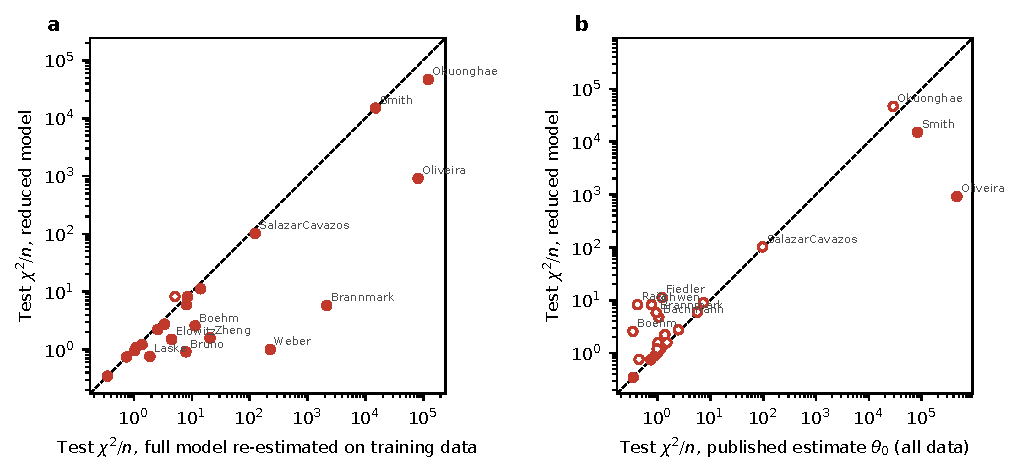
\includegraphics[width=\textwidth]{figures/fig3_validation.pdf}
\caption{\textbf{Prediction of held-out experiments with real data.} Mean squared noise-scaled residual ($\chi^2/n$) on the test experiments for the reduced model (vertical axis) against \textbf{a}, the full model re-estimated on the same training experiments ($n=25$ problems with $p\le 60$) and \textbf{b}, the published estimate $\theta_0$, which was obtained using all data including the test experiments ($n=29$). Filled symbols: reduced model within 5\% of, or better than, the reference; open symbols: worse. Points below the dashed diagonal mean that the reduced model predicts better. Problems with noise-free benchmark data (test $\chi^2/n$ of $\theta_0$ below 0.01; Giordano, Perelson, Rahman) are omitted. Names are shown for points away from the diagonal.}
\label{fig:validation}
\end{figure}

\subsection*{Robustness to the size of parameter changes}\label{sec:patterns}

Admissibility is decided with perturbations of $\pm$5\%. To determine how far the conclusion extends, we kept each final subset fixed and repeated the evaluation with perturbations of $\pm$1, 5, 10, 20, 30, 40 and 50\% (15 scenarios per level, same random seed at every level, so that the $\pm$5\% level reproduces the selection). We classified the behaviour of the median $e_{\mathrm{fit}}$ into four patterns: A, admissible at all levels; B, admissible up to at least $\pm$20\% and not thereafter; C, irregular (failing and then passing again); D, failing at $\pm$10\% or less.

All 32 admissible problems were evaluated. Twenty-seven follow pattern A (Fig.~\ref{fig:robustness}): their median $e_{\mathrm{fit}}$ stays below the threshold up to $\pm$50\%, typically varying by only a few percentage points across levels. Four follow pattern B: Armistead, whose error grows steadily from 3\% at $\pm$1\% to 63\% at $\pm$50\%, and Bertozzi, Blasi and Elowitz, which are close to the threshold already at $\pm$5\% and cross it between $\pm$20\% and $\pm$30\%. Lucarelli is the only case of pattern C: its median error stays between 43\% and 47\% at all levels, that is, on the threshold rather than clearly above or below it. No problem follows pattern D. The reductions therefore remain valid well beyond the $\pm$5\% used for selection in most problems, whereas problems that are admissible only with a small margin at $\pm$5\% are those that lose admissibility for large changes.

\begin{figure}[t]
\centering
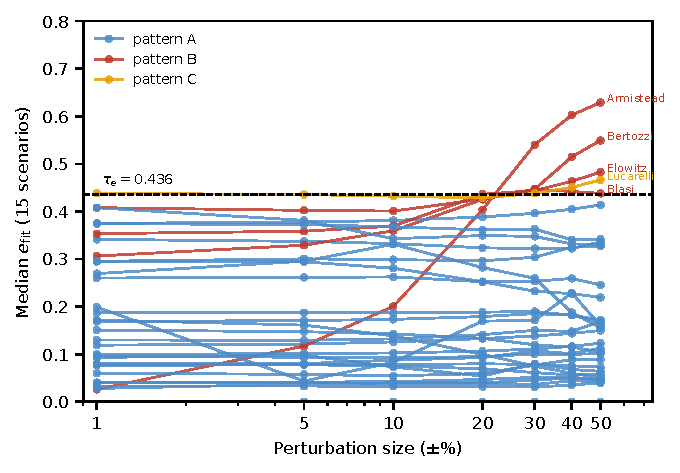
\includegraphics[width=0.66\textwidth]{figures/fig4_robustness.pdf}
\caption{\textbf{Robustness of the selected subsets to the size of parameter changes.} Median relative error after re-estimation ($e_{\mathrm{fit}}$, 15 random scenarios per level) as a function of the perturbation size, for the final subset of each of the 32 admissible problems. Colours indicate the robustness pattern: A, admissible at all levels (blue, $n=27$); B, admissible up to at least $\pm$20\% (red, $n=4$); C, irregular (orange, $n=1$). The dashed line marks the admissibility threshold $\tau_e=0.436$.}
\label{fig:robustness}
\end{figure}

\subsection*{Sensitivity to method settings and computational cost}\label{sec:settings}

The method depends on a finite-difference step $\delta$, integrator tolerances, the perturbation size used for admissibility and four thresholds ($\tau_R$, $\tau_\kappa$, $\tau_{\mathrm{VIF}}$, $\tau_e$). We re-ran the complete method on the 26 small and medium problems changing one setting at a time (Table~\ref{tab:settings}). The selected subset was identical to the baseline in all 26 problems for $\delta=0.1\%$ and $5\%$, for perturbations of $\pm$1\% and $\pm$10\%, and for $\tau_R$ between 0.80 and 0.95, and in 25 of 26 with tighter integrator tolerances; admissibility decisions changed in at most one problem (Perelson at $\pm$1\%, where the perturbed output change falls below the numerical noise floor). The $\kappa$/VIF threshold changed the subset in three or four problems without changing the number of admissible problems. As expected, the error threshold $\tau_e$ has the largest influence: requiring $e_{\mathrm{fit}}\le 10\%$ leaves 22 admissible problems with a mean of 3.6 biological parameters, whereas $\tau_e$ between 0.30 and 0.50 gives 25 admissible problems with 2.1--2.4 parameters. The threshold therefore acts as an accuracy--parsimony trade-off that the user can set; we also examined single-parameter subsets: in ten problems one parameter reached the threshold at $\pm$5\%, but in the synthetic prediction experiment the selected pair predicted better in six of nine comparable problems, which supports the minimum size of two.

The dominant cost is the computation of $J$ (2$p$ simulations) and of the stage-2 ordering ($p$ simulations), so the number of simulations grows linearly with the number of parameters, and all of them are independent and can run in parallel; the selection, condition-number tests, backward elimination and the first-order version of $e_{\mathrm{fit}}$ only use linear algebra on $J$. On a four-core server, these simulations took less than 40~s for all but two of the problems we timed, 2~min for Lang (294 parameters) and 68~min for Chen (155 parameters, 35~s per simulation). On state trajectories, the 4,231-parameter Froehlich model required 12,693 simulations and 2.6~h. For models of this size on measured outputs, forward or adjoint sensitivity equations\cite{bib13} compute $J$ at the cost of a few simulations.

\begin{table}[t]
\caption{\textbf{Sensitivity of the selection to the method settings.} The complete method was re-run on 26 problems changing one setting at a time (baseline: $\delta=1\%$, perturbation $\pm$5\%, $\tau_R=0.89$, $\tau_\kappa=\tau_{\mathrm{VIF}}=10$, $\tau_e=0.436$). Same $S$, number of problems in which the selected subset is identical to the baseline; $\overline{|S|}$, mean number of selected biological parameters among admissible problems.}
\label{tab:settings}
\centering
\small
\begin{tabular}{@{}lccc@{}}
\toprule
Setting & Admissible & $\overline{|S|}$ & Same $S$ \\
\midrule
Baseline & 25 & 2.16 & 26/26 \\
$\delta=0.1\%$ / $\delta=5\%$ & 25 / 25 & 2.16 & 26/26 / 26/26 \\
Tolerances $10^{-9}/10^{-12}$ / $10^{-6}/10^{-8}$ & 25 / 25 & 2.16 & 25/26 / 26/26 \\
Perturbation $\pm$1\% / $\pm$10\% & 24 / 25 & 2.16 & 26/26 / 26/26 \\
$\tau_R=0.80$ / $0.85$ / $0.95$ & 25 & 2.16 & 26/26 \\
$\tau_\kappa=\tau_{\mathrm{VIF}}=5$ & 25 & 2.16 & 23/26 \\
$\tau_\kappa=\tau_{\mathrm{VIF}}=30$ & 25 & 2.16 & 22/26 \\
$\tau_e=0.10$ & 22 & 3.64 & 12/26 \\
$\tau_e=0.20$ & 24 & 2.71 & 17/26 \\
$\tau_e=0.30$ & 25 & 2.44 & 20/26 \\
$\tau_e=0.50$ & 25 & 2.08 & 24/26 \\
\botrule
\end{tabular}
\end{table}

\subsection*{Formal guarantees}\label{sec:formal}

Table~\ref{tab:theorems} lists the mathematical statements on which the method relies and that are verified in Lean~4 with Mathlib; Supplementary Table~S3 gives the name of each formal theorem. None of the proofs uses unproved assumptions (\texttt{sorry}) or additional axioms. Two statements are central to the method:

\begin{theorem}\label{thm:cos}
For vectors $d\neq 0$ and $b\neq 0$ in a real inner-product space, $\min_{\lambda\in\mathbb{R}}\|d-\lambda b\|/\|d\| = \sqrt{1-\cos^2(d,b)}$.
\end{theorem}

\begin{theorem}\label{thm:prune}
Let $\mathcal{A}$ be any admissibility predicate on finite sets and $S$ an admissible set. Backward elimination (removing one element at a time whenever the remaining set is still admissible, until no element can be removed) returns an admissible subset of $S$ from which no element can be removed without losing admissibility.
\end{theorem}

Theorem~\ref{thm:cos} justifies the threshold $\tau_e$: an error of at most $\sqrt{1-c^2}$ after re-estimation is the natural counterpart of a cosine similarity of at least $c$. Theorem~\ref{thm:prune} gives the precise sense in which the selected subsets are minimal: no parameter can be removed, although a different, smaller admissible subset that is not contained in the result may exist. The other verified statements cover the remaining steps: re-estimating more parameters never increases the fitting error and $e_{\mathrm{fit}}\le e_{\mathrm{rel}}$; the selection keeps $\kappa$ and VIF below their thresholds and permanently discarding a rejected candidate is correct because both quantities can only increase when parameters are added; $\kappa$ and VIF bounds imply unique and stable least-squares estimates; error bounds on the states transfer to the measured outputs, including logarithmic transformations; and the first-order version of $e_{\mathrm{fit}}$ used for the largest models differs from the exact one by a second-order term. The verification is local: it does not prove that a subset remains adequate far from $\theta_0$, which is assessed empirically above.

\begin{table}[t]
\caption{\textbf{Formally verified statements (Lean~4/Mathlib).} Each statement is proved without unproved assumptions or additional axioms. The corresponding formal theorem names are given in Supplementary Table~S3.}
\label{tab:theorems}
\centering
\small
\begin{tabular}{@{}p{0.30\textwidth}p{0.64\textwidth}@{}}
\toprule
Step of the method & Verified statement \\
\midrule
Energy and $R_{\mathrm{var}}$ & $E_j=(J^\top J)_{jj}$; the total energy is the sum of retained and discarded energy; the first-order output change caused by discarded parameters is bounded by their energy \\
Sensitivities of the ODE & For $C^1$ vector fields, solutions depend differentiably on parameters and initial conditions, and the sensitivity solves the variational equation \\
Greedy selection & The returned subset satisfies $\kappa\le\tau_\kappa$ and $\mathrm{VIF}\le\tau_{\mathrm{VIF}}$; rejected candidates would still violate the test with the final subset \\
Identifiability & $\kappa$ and VIF bounds imply uniqueness and stability of least-squares estimates of the retained parameters \\
Admissibility threshold & Theorem~\ref{thm:cos} (minimum error after rescaling equals $\sqrt{1-\cos^2}$) \\
Re-estimation & Adding parameters to the re-estimated set cannot increase the fitting error; $e_{\mathrm{fit}}\le e_{\mathrm{rel}}$ \\
Backward elimination & Theorem~\ref{thm:prune} (minimality with respect to inclusion) \\
Measured outputs & Error bounds on states transfer to outputs $y_i=h(g_i(x))/\sigma_i$ with Lipschitz observables; $\log$ and $\log_{10}$ are Lipschitz on $[c,\infty)$ \\
First-order $e_{\mathrm{fit}}$ & The linearised fitting error never exceeds the rescaled error and differs from the exact one by at most a second-order term \\
Model assumptions & For 22 of the benchmark models translated from SBML, the vector field is smooth, solutions exist on the simulated horizon and concentrations remain non-negative \\
\botrule
\end{tabular}
\end{table}

\section*{Discussion}\label{sec:discussion}

The central finding is that, for most published systems biology models with real data, the measured outputs can be reproduced by re-estimating only two biological parameters plus the measurement calibration parameters, and that such reduced models predict held-out experiments as well as or better than the full models. This is consistent with the sloppy-model picture\cite{bib15}, but it is a stronger and more practical statement: it refers to the outputs that were actually measured, under the actual experimental conditions and noise levels, and it is checked by re-estimation and external validation rather than inferred from the sensitivity spectrum alone. The two-stage design reflects a practical observation: ranking by local sensitivity energy (stage~1) was sufficient in only seven problems, whereas ranking by finite-perturbation effects (stage~2) was needed in most. Energy measures how strongly a parameter moves the outputs, not whether adjusting it can compensate for changes in other parameters; the admissibility test, which re-estimates the subset, is what decides.

The method complements existing approaches. Profile likelihood\cite{bib24,bib25} and likelihood-based observability analysis\cite{bib17} assess identifiability after calibration and require repeated optimisation in the full parameter space; Bayesian approaches such as approximate Bayesian computation\cite{bib20} require many more simulations. Global sensitivity analysis\cite{bib26,bib23} ranks parameters but does not produce a non-redundant subset validated by re-estimation, and structural identifiability analysis\cite{bib4,bib10,bib29} addresses ideal noise-free data rather than a given experimental design. Model-order reduction methods such as balanced truncation\cite{bib22,bib1} reduce the number of state variables rather than parameters. Our method requires a number of simulations that grows linearly with the number of parameters, is applied before calibration and returns a concrete subset with documented fidelity, prediction and robustness.

Several limitations should be noted. First, the analysis is local: sensitivities are computed at the published estimate $\theta_0$, which is assumed to be a good fit to the data, and admissibility is tested with perturbations around it. The robustness analysis shows that most reductions remain valid for changes of up to $\pm$50\%, but this cannot be assumed for every model, and problems that are admissible with a small margin at $\pm$5\% (Bertozzi, Blasi, Elowitz, Lucarelli) are those that lose admissibility for larger changes. Second, the method assumes that the model is smooth in the parameters, that the measurement noise is Gaussian with the standard deviations recorded in the benchmark and that the calibration parameters can always be re-estimated; in three problems the recorded noise levels do not match the scatter of the data, and in problems with many calibration parameters (Bachmann, Raimundez) the reduced problem is still sizeable. Third, for the eight problems with the most expensive simulations the fitting error was computed to first order; the verified bounds show that the difference from the exact error is of second order in the perturbation, but it was not quantified numerically for each model. Fourth, one benchmark problem with 9,169 experimental conditions was too expensive to analyse on its measured outputs with finite differences, and two problems had no admissible subset: Beer, and Crauste, whose model has no solution on the measured horizon for parameter changes of 1\%. Finally, the formal verification covers the mathematical steps of the method and the regularity of the translated models, not the numerical simulator itself; we cross-checked our simulations against the reference simulations distributed with the benchmark.

The social cognitive theory model, which motivated this work, illustrates the same behaviour outside molecular biology: with a single measured output the full estimation problem is ill-posed, and the conditioning test identifies two parameters that carry the information in that output. In practice, the method can be used as a preprocessing step: before calibrating a large model, select the few biological parameters that the data can inform, re-estimate them together with the calibration parameters, keep the rest at literature values, and verify the reduced model on held-out experiments. The threshold $\tau_e$ provides an explicit trade-off between accuracy and parsimony. Natural extensions include computing $J$ with forward or adjoint sensitivity equations for genome-scale models, combining sensitivities at several operating points, and using the selected subsets to guide experimental design\cite{bib28}.

\section*{Methods}\label{sec:methods}

\subsection*{Models, data and simulation}

We used the problems of the PEtab benchmark collection\cite{bib31,bib27} that provide real measurements, an SBML model and nominal parameter values (34 problems; Table~\ref{tab:benchmark}). Each problem specifies the observables $g_i$, their transformation $h$ (linear, $\log$ or $\log_{10}$), the noise standard deviation $\sigma_i$ of each measurement, the experimental conditions (parameter or initial-value overrides) and, where applicable, pre-equilibration conditions. Models were simulated with libRoadRunner\cite{bib32} (CVODE, relative and absolute tolerances $10^{-7}$ and $10^{-10}$). Initial assignments that depend on parameters were re-evaluated for every parameter vector, condition-specific overrides were applied before simulation, pre-equilibration was run to steady state before the main simulation, and models with discontinuous inputs were integrated piecewise between discontinuities. Simulated observables were compared with the reference simulations distributed with the benchmark wherever available (Supplementary Note).

\subsection*{Social cognitive theory model}

The model\cite{bib34,bib35} has six states $x_i$ (constructs of social cognitive theory\cite{bib3}) and obeys $\dot x=A(\theta)x+B(\theta)u$, $y=x_4$ (behaviour), with $A_{ii}=-1/\tau_i$, $A_{ij}=\beta_{ij}/\tau_i$ for the ten couplings $\beta_{14},\beta_{21},\beta_{25},\beta_{31},\beta_{34},\beta_{42},\beta_{43},\beta_{45},\beta_{46},\beta_{54}$, and input gains $\gamma_{33},\gamma_{35},\gamma_{36},\gamma_{57},\gamma_{64},\gamma_{68}$ divided by the time constant of the receiving construct (22 parameters). Nominal values are the differential-evolution estimates reported previously for this model\cite{bib35}. Six input conditions, each a unit step on one of the six inputs, were simulated from $x(0)=0$ on $[0,10]$ with a fourth-order Runge--Kutta scheme on 80 equally spaced points (480 output values; 2,880 values when all states are used). All parameters are model parameters, the outputs are not scaled by noise, and all other settings are as for the benchmark problems.

\subsection*{Measured outputs and parameter classes}

For a parameter vector $\theta\in\mathbb{R}^p$ (in the units of the benchmark, excluding noise parameters), the vector of scaled outputs is $y(\theta)\in\mathbb{R}^m$ with entries
\begin{equation}
y_i(\theta)=\frac{h\big(g_i(x(t_i;\theta,c_i),\theta)\big)}{\sigma_i},\qquad i=1,\dots,m,
\label{eq:outputs}
\end{equation}
where $x(t;\theta,c)$ is the state trajectory under condition $c$ and $(t_i,c_i)$ are the time and condition of measurement $i$. Parameters that appear in the SBML model are biological ($\Theta_B$); parameters that appear only in the observation functions and not in the model or the condition table (scalings and offsets) are calibration parameters ($\Theta_C$). Only biological parameters are candidates for selection; calibration parameters are always re-estimated.

\subsection*{Sensitivities, energy and conditioning}

The relative sensitivity matrix $J\in\mathbb{R}^{m\times p}$ is computed by central differences,
\begin{equation}
J_{:,j}=\frac{y(\theta_0+\delta\theta_{0,j}e_j)-y(\theta_0-\delta\theta_{0,j}e_j)}{2\delta},
\label{eq:jac}
\end{equation}
which approximates $\partial y/\partial\log\theta_j$. The energy of parameter $j$ is $E_j=\|J_{:,j}\|^2=(J^\top J)_{jj}$ and the fraction of energy captured by a subset $S\subseteq\Theta_B$ is $R_{\mathrm{var}}(S)=\sum_{j\in S}E_j/\sum_{j\in\Theta_B}E_j$. For a subset $S$, the columns of $J_S$ are normalised to unit length, $Z=J_S\,\mathrm{diag}(\|J_{:,j}\|)^{-1}$; the condition number is $\kappa(S)=\sigma_{\max}(Z)/\sigma_{\min}(Z)$ and the largest variance inflation factor is $\mathrm{VIF}(S)=\max_j[(Z^\top Z)^{-1}]_{jj}$\cite{bib5,bib9}. Normalisation removes differences of scale between parameters, so that $\kappa$ and VIF measure only the angles between sensitivity directions.

\subsection*{Selection}

\emph{Greedy selection.} Candidates are visited in a given order. A candidate $j$ is accepted if $\kappa(S\cup\{j\})\le\tau_\kappa$ and $\mathrm{VIF}(S\cup\{j\})\le\tau_{\mathrm{VIF}}$; otherwise it is discarded permanently. Because $\kappa$ and VIF can only increase when columns are added, a discarded candidate would also be rejected later. \emph{Stage~1} visits biological parameters in decreasing order of $E_j$ and stops when $R_{\mathrm{var}}(S)\ge\tau_R$. \emph{Stage~2}, used if the stage-1 subset is not admissible, visits biological parameters in decreasing order of the finite-perturbation effect $s_j=\|y(\theta_0+\eta\theta_{0,j}e_j)-y(\theta_0)\|$ and stops at the first admissible subset. \emph{Backward elimination} visits the parameters of the selected subset and removes each one whose removal leaves the subset admissible.

\subsection*{Admissibility and re-estimation}

Admissibility is evaluated on $N$ random scenarios $\theta^{(k)}=\theta_0\odot(1+\varepsilon u^{(k)})$, with $u^{(k)}$ uniform in $[-1,1]^p$. For each scenario let $\Delta y_{\mathrm{full}}=y(\theta^{(k)})-y(\theta_0)$. The relative error without re-estimation is $e_{\mathrm{rel}}=\|\Delta y_{\mathrm{full}}-\Delta y_S\|/\|\Delta y_{\mathrm{full}}\|$, where $\Delta y_S$ is the output change when only the parameters in $S\cup\Theta_C$ take their scenario values, and the cosine similarity is $\cos\Delta=\langle\Delta y_{\mathrm{full}},\Delta y_S\rangle/(\|\Delta y_{\mathrm{full}}\|\|\Delta y_S\|)$. The relative error after re-estimation is
\begin{equation}
e_{\mathrm{fit}}=\min_{\theta_{S},\theta_C}\frac{\|y(\theta_S,\theta_C,\theta_{0,\overline{S}})-y(\theta^{(k)})\|}{\|\Delta y_{\mathrm{full}}\|},
\label{eq:efit}
\end{equation}
where $\theta_{0,\overline{S}}$ denotes the nominal values of all other biological parameters. The minimisation is carried out in $\log|\theta|$ within $[|\theta_0|/10,\,10|\theta_0|]$ by a trust-region reflective least-squares method (SciPy\cite{bib33}, at most $100(|S|+|\Theta_C|+1)$ function evaluations), from two starting points (the scenario value and $\theta_0$); the error without re-estimation is also included, so that $e_{\mathrm{fit}}\le e_{\mathrm{rel}}$. Scenarios whose output change is below $\max(10^{-10}\|y(\theta_0)\|,10^{-6})$ are discarded. $S$ is admissible if $|S|\ge k_{\min}$ and the median of $e_{\mathrm{fit}}$ over the scenarios is at most $\tau_e=\sqrt{1-c^2}$. For the eight problems in which the cost of simulation made repeated re-estimation impractical (marked in Table~\ref{tab:benchmark}), the first-order version $\min_c\|\Delta y_{\mathrm{full}}-J_{S\cup\Theta_C}c\|/\|\Delta y_{\mathrm{full}}\|$ was used.

\subsection*{Settings}

Unless stated otherwise: $\delta=0.01$; $\eta=0.1$; $\tau_R=0.89$; $\tau_\kappa=\tau_{\mathrm{VIF}}=10$; $N=15$ scenarios; $\varepsilon=0.05$; random seed 42; $c=0.9$, so $\tau_e=0.436$; $k_{\min}=2$. The sensitivity analysis (Table~\ref{tab:settings}) changed one setting at a time on the 26 problems that could be re-run completely in reasonable time.

\subsection*{External validation}

Measurements were split into training and test sets by experimental condition (every third condition after sorting, or the second of two conditions, used for testing) or, for problems with a single condition, by time (the last third of the distinct measurement times). Parameters that only affect test conditions were excluded from re-estimation. The reduced model (re-estimating $S\cup\Theta_C$) and the full model (re-estimating all parameters; only for $p\le 60$ because of cost) were fitted to the training data from $\theta_0$ with the same least-squares method and bounds, and evaluated by the mean squared noise-scaled residual $\chi^2/n=\frac{1}{n}\sum_{i\in\mathrm{test}}(y_i(\hat\theta)-\tilde y_i)^2$, where $\tilde y_i$ are the scaled measurements. In the synthetic experiment, the truth $\theta^\ast$ had each parameter drawn uniformly within $\pm$20\% of $\theta_0$, data were simulated with Gaussian noise of standard deviation $\sigma_i$, and $e_{\mathrm{pred}}=\|y_{\mathrm{test}}(\hat\theta)-y_{\mathrm{test}}(\theta^\ast)\|/\|y_{\mathrm{test}}(\theta^\ast)-y_{\mathrm{test}}(\theta_0)\|$; the effect of the parameter change was considered larger than the noise when $\chi^2/n$ of $\theta_0$ on the synthetic test data was at least 2.

\subsection*{Robustness patterns}

For each admissible problem, the final subset was kept fixed and $e_{\mathrm{fit}}$ was evaluated at perturbation sizes $\varepsilon\in\{0.01,0.05,0.10,0.20,0.30,0.40,0.50\}$ with 15 scenarios per level, using the same random seed at each level. Patterns were assigned from the median $e_{\mathrm{fit}}$ at each level as described in Results. As in the selection, $e_{\mathrm{fit}}$ was computed to first order for the problems marked in Table~\ref{tab:benchmark}. For Chen, between 7 and 13 of the 15 scenarios per level could be simulated; the remaining scenarios failed to integrate and were discarded.

\subsection*{Formal verification}

The formal development uses Lean~4 (version 4.23.0) and Mathlib\cite{bib19,bib21}. Model regularity (smoothness of the vector field, existence of solutions on the simulated horizon and non-negativity of concentrations) was verified for 22 benchmark models by translating their SBML rate laws into Lean expressions and applying verified checkers. All files compile without \texttt{sorry}, and \texttt{\#print axioms} reports only the standard axioms of Lean's logic (\texttt{propext}, \texttt{Classical.choice}, \texttt{Quot.sound}).

\subsection*{Use of large language models}

An AI assistant (Claude, Anthropic) was used to help write and debug analysis code and Lean proofs and to edit the manuscript text. All code, proofs and results were checked by the authors, who take full responsibility for the content.

\backmatter

\bmhead{Data availability}
The PEtab benchmark problems analysed in this study are publicly available in the Benchmark-Models-PEtab collection (\url{https://github.com/Benchmarking-Initiative/Benchmark-Models-PEtab}). The social cognitive theory model is provided as Python code in the repository below. All results generated in this study (selected subsets, validation, robustness and sensitivity analyses) are available at \url{https://github.com/monicammr/archivos} and will be archived on Zenodo upon acceptance.

\bmhead{Code availability}
The Python analysis code and the Lean~4 formal development are available at \url{https://github.com/monicammr/archivos} and will be archived on Zenodo upon acceptance.

\bmhead{Acknowledgements}
The authors thank Escuela Superior Polit\'ecnica del Litoral (ESPOL) for institutional support.

\bmhead{Author contributions}
M.M.R. and C.S. conceived the study and designed the method. M.M.R. wrote the software and the formal proofs, performed the analyses and wrote the first draft. C.S., C.M. and A.A. supervised the work, contributed to the validation of the results and revised the manuscript. All authors reviewed and approved the final manuscript.

\bmhead{Funding}
This research received no external funding.

\bmhead{Additional information}
\textbf{Competing interests:} The authors declare no competing interests.\\
\textbf{Correspondence} and requests for materials should be addressed to M.M.R.\\
\textbf{Supplementary information} accompanies this paper (Supplementary Tables S1--S3 and Supplementary Note).

\begin{thebibliography}{27}
\expandafter\ifx\csname url\endcsname\relax
  \def\url#1{\burl{#1}}\fi
\expandafter\ifx\csname urlprefix\endcsname\relax\def\urlprefix{URL }\fi
\providecommand{\bibinfo}[2]{#2}
\providecommand{\eprint}[2][]{\url{#2}}
\providecommand{\doi}[1]{\url{https://doi.org/#1}}
\bibcommenthead

\bibitem{bib16}
\bibinfo{author}{Kholodenko, B.~N.}
\newblock \bibinfo{title}{Cell-signalling dynamics in time and space}.
\newblock \emph{\bibinfo{journal}{Nature Reviews Molecular Cell Biology}}
  \textbf{\bibinfo{volume}{7}}, \bibinfo{pages}{165--176}
  (\bibinfo{year}{2006}).

\bibitem{bib4}
\bibinfo{author}{Bellman, R.} \& \bibinfo{author}{{\AA}str{\"o}m, K.~J.}
\newblock \bibinfo{title}{On structural identifiability}.
\newblock \emph{\bibinfo{journal}{Mathematical Biosciences}}
  \textbf{\bibinfo{volume}{7}}, \bibinfo{pages}{329--339}
  (\bibinfo{year}{1970}).

\bibitem{bib10}
\bibinfo{author}{Chi{\c{s}}, O.-T.}, \bibinfo{author}{Banga, J.~R.} \&
  \bibinfo{author}{Balsa-Canto, E.}
\newblock \bibinfo{title}{Structural identifiability of systems biology models:
  A critical comparison of methods}.
\newblock \emph{\bibinfo{journal}{PLOS ONE}} \textbf{\bibinfo{volume}{6}},
  \bibinfo{pages}{e27755} (\bibinfo{year}{2011}).

\bibitem{bib29}
\bibinfo{author}{Villaverde, A.~F.}, \bibinfo{author}{Barreiro, A.} \&
  \bibinfo{author}{Papachristodoulou, A.}
\newblock \bibinfo{title}{Structural identifiability of dynamic systems biology
  models: A critical comparison of analysis methods}.
\newblock \emph{\bibinfo{journal}{PLOS Computational Biology}}
  \textbf{\bibinfo{volume}{12}}, \bibinfo{pages}{e1004873}
  (\bibinfo{year}{2016}).

\bibitem{bib24}
\bibinfo{author}{Raue, A.} \emph{et~al.}
\newblock \bibinfo{title}{Structural and practical identifiability analysis of
  partially observed dynamical models by exploiting the profile likelihood}.
\newblock \emph{\bibinfo{journal}{Bioinformatics}}
  \textbf{\bibinfo{volume}{25}}, \bibinfo{pages}{1923--1929}
  (\bibinfo{year}{2009}).

\bibitem{bib25}
\bibinfo{author}{Raue, A.}, \bibinfo{author}{Kreutz, C.},
  \bibinfo{author}{Theis, F.~J.} \& \bibinfo{author}{Timmer, J.}
\newblock \bibinfo{title}{Joining forces of {Bayesian} and frequentist
  methodology: A study for inference in the presence of non-identifiability}.
\newblock \emph{\bibinfo{journal}{Philosophical Transactions of the Royal
  Society A}} \textbf{\bibinfo{volume}{371}}, \bibinfo{pages}{20110544}
  (\bibinfo{year}{2013}).

\bibitem{bib17}
\bibinfo{author}{Kreutz, C.}, \bibinfo{author}{Raue, A.} \&
  \bibinfo{author}{Timmer, J.}
\newblock \bibinfo{title}{Likelihood based observability analysis and
  confidence intervals for predictions of dynamic models}.
\newblock \emph{\bibinfo{journal}{BMC Systems Biology}}
  \textbf{\bibinfo{volume}{6}}, \bibinfo{pages}{120} (\bibinfo{year}{2012}).

\bibitem{bib31}
\bibinfo{author}{Hass, H.} \emph{et~al.}
\newblock \bibinfo{title}{Benchmark problems for dynamic modeling of intracellular processes}.
\newblock \emph{\bibinfo{journal}{Bioinformatics}} \textbf{\bibinfo{volume}{35}}, \bibinfo{pages}{3073--3082} (\bibinfo{year}{2019}).

\bibitem{bib12}
\bibinfo{author}{Fr{\"o}hlich, F.}, \bibinfo{author}{Loos, C.} \&
  \bibinfo{author}{Hasenauer, J.}
\newblock \bibinfo{title}{Scalable parameter estimation for genome-scale
  biochemical reaction networks}.
\newblock \emph{\bibinfo{journal}{PLOS Computational Biology}}
  \textbf{\bibinfo{volume}{14}}, \bibinfo{pages}{e1005991}
  (\bibinfo{year}{2018}).

\bibitem{bib15}
\bibinfo{author}{Gutenkunst, R.~N.} \emph{et~al.}
\newblock \bibinfo{title}{Universally sloppy parameter sensitivities in systems
  biology models}.
\newblock \emph{\bibinfo{journal}{PLOS Computational Biology}}
  \textbf{\bibinfo{volume}{3}}, \bibinfo{pages}{e189} (\bibinfo{year}{2007}).

\bibitem{bib26}
\bibinfo{author}{Saltelli, A.}, \bibinfo{author}{Tarantola, S.},
  \bibinfo{author}{Campolongo, F.} \& \bibinfo{author}{Ratto, M.}
\newblock \emph{\bibinfo{title}{Sensitivity analysis in practice: A guide to
  assessing scientific models}}  (\bibinfo{publisher}{Wiley},
  \bibinfo{year}{2004}).

\bibitem{bib23}
\bibinfo{author}{Morris, M.~D.}
\newblock \bibinfo{title}{Factorial sampling plans for preliminary
  computational experiments}.
\newblock \emph{\bibinfo{journal}{Technometrics}}
  \textbf{\bibinfo{volume}{33}}, \bibinfo{pages}{161--174}
  (\bibinfo{year}{1991}).

\bibitem{bib5}
\bibinfo{author}{Belsley, D.~A.}, \bibinfo{author}{Kuh, E.} \&
  \bibinfo{author}{Welsch, R.~E.}
\newblock \emph{\bibinfo{title}{Regression diagnostics: Identifying influential
  data and sources of collinearity}}  (\bibinfo{publisher}{Wiley},
  \bibinfo{year}{1980}).

\bibitem{bib9}
\bibinfo{author}{Brun, R.}, \bibinfo{author}{Reichert, P.} \&
  \bibinfo{author}{K{\"u}nsch, H.~R.}
\newblock \bibinfo{title}{Practical identifiability analysis of large
  environmental simulation models}.
\newblock \emph{\bibinfo{journal}{Water Resources Research}}
  \textbf{\bibinfo{volume}{37}}, \bibinfo{pages}{1015--1030}
  (\bibinfo{year}{2001}).

\bibitem{bib3}
\bibinfo{author}{Bandura, A.}
\newblock \emph{\bibinfo{title}{Social Foundations of Thought and Action: A
  Social Cognitive Theory}}  (\bibinfo{publisher}{Prentice-Hall},
  \bibinfo{year}{1986}).

\bibitem{bib34}
\bibinfo{author}{Mart\'in, C.~A.}, \bibinfo{author}{Rivera, D.~E.}, \bibinfo{author}{Aguirre, A.~A.} \& \bibinfo{author}{Salazar, C.~A.}
\newblock \bibinfo{title}{Dynamic modeling of social cognitive theory constructs in physical activity interventions}.
\newblock \emph{\bibinfo{journal}{J. Process Control}} \textbf{\bibinfo{volume}{75}}, \bibinfo{pages}{1--13} (\bibinfo{year}{2019}).

\bibitem{bib35}
\bibinfo{author}{Miranda~R., M.}, \bibinfo{author}{Salazar~L., C.}, \bibinfo{author}{Mart\'in~M., C.} \& \bibinfo{author}{Aguirre~A., A.}
\newblock \bibinfo{title}{Hybrid estimation of dynamic behavioral models using differential evolution and grey-box refinement}.
\newblock In \emph{\bibinfo{booktitle}{2025 IEEE Ninth Ecuador Technical Chapters Meeting (ETCM)}}, \bibinfo{pages}{1--7} (\bibinfo{publisher}{IEEE}, \bibinfo{year}{2025}).

\bibitem{bib27}
\bibinfo{author}{Schmiester, L.} \emph{et~al.}
\newblock \bibinfo{title}{{PEtab}---interoperable specification of parameter
  estimation problems in systems biology}.
\newblock \emph{\bibinfo{journal}{PLOS Computational Biology}}
  \textbf{\bibinfo{volume}{17}}, \bibinfo{pages}{e1008646}
  (\bibinfo{year}{2021}).

\bibitem{bib19}
\bibinfo{author}{de~Moura, L.} \& \bibinfo{author}{Ullrich, S.}
\newblock \bibinfo{title}{The {Lean} 4 theorem prover and programming language}.
\newblock In \emph{\bibinfo{booktitle}{Automated Deduction -- CADE 28}}, \bibinfo{series}{Lecture Notes in Computer Science} \textbf{\bibinfo{volume}{12699}}, \bibinfo{pages}{625--635} (\bibinfo{publisher}{Springer}, \bibinfo{year}{2021}).

\bibitem{bib21}
\bibinfo{author}{{Mathlib Community}}.
\newblock \bibinfo{title}{The {Lean} mathematical library}.
\newblock \bibinfo{howpublished}{Proceedings of the 9th ACM SIGPLAN
  International Conference on Certified Programs and Proofs}
  (\bibinfo{year}{2020}).

\bibitem{bib13}
\bibinfo{author}{Fr{\"o}hlich, F.}, \bibinfo{author}{Weindl, D.} \&
  \bibinfo{author}{Hasenauer, J.}
\newblock \bibinfo{title}{{AMICI}: High-performance sensitivity analysis for
  large ordinary differential equation models}.
\newblock \emph{\bibinfo{journal}{Bioinformatics}}
  \textbf{\bibinfo{volume}{37}}, \bibinfo{pages}{3676--3677}
  (\bibinfo{year}{2021}).

\bibitem{bib20}
\bibinfo{author}{Liepe, J.} \emph{et~al.}
\newblock \bibinfo{title}{A framework for parameter estimation and model
  selection in systems biology using approximate {Bayesian} computation}.
\newblock \emph{\bibinfo{journal}{Nature Protocols}}
  \textbf{\bibinfo{volume}{9}}, \bibinfo{pages}{439--456}
  (\bibinfo{year}{2014}).

\bibitem{bib22}
\bibinfo{author}{Moore, B.~C.}
\newblock \bibinfo{title}{Principal component analysis in linear systems:
  Controllability, observability, and model reduction}.
\newblock \emph{\bibinfo{journal}{IEEE Transactions on Automatic Control}}
  \textbf{\bibinfo{volume}{26}}, \bibinfo{pages}{17--32}
  (\bibinfo{year}{1981}).

\bibitem{bib1}
\bibinfo{author}{Antoulas, A.~C.}
\newblock \emph{\bibinfo{title}{Approximation of large-scale dynamical
  systems}}  (\bibinfo{publisher}{SIAM}, \bibinfo{year}{2005}).

\bibitem{bib28}
\bibinfo{author}{Transtrum, M.~K.} \& \bibinfo{author}{Qiu, P.}
\newblock \bibinfo{title}{Optimal experiment selection for parameter estimation
  in biological differential equation models}.
\newblock \emph{\bibinfo{journal}{BMC Bioinformatics}}
  \textbf{\bibinfo{volume}{13}}, \bibinfo{pages}{181} (\bibinfo{year}{2012}).

\bibitem{bib32}
\bibinfo{author}{Welsh, C.} \emph{et~al.}
\newblock \bibinfo{title}{libRoadRunner 2.0: a high performance {SBML} simulation and analysis library}.
\newblock \emph{\bibinfo{journal}{Bioinformatics}} \textbf{\bibinfo{volume}{39}}, \bibinfo{pages}{btac770} (\bibinfo{year}{2023}).

\bibitem{bib33}
\bibinfo{author}{Virtanen, P.} \emph{et~al.}
\newblock \bibinfo{title}{{SciPy} 1.0: fundamental algorithms for scientific computing in {Python}}.
\newblock \emph{\bibinfo{journal}{Nat. Methods}} \textbf{\bibinfo{volume}{17}}, \bibinfo{pages}{261--272} (\bibinfo{year}{2020}).

\end{thebibliography}


\end{document}
